\chapter{Měření}

\section{Přesnost}
\section{Reprodukovatelnost}
Reprodukovatelnost mechanismu je po přesnosti pozicování dalším z klíčovým parametrem. Přesnost a reprodukovatelnost jsou spolu úzce spojeny. Reprodukovatelnost je definována jako schopnost mechanismu vracet se zpet na dané místo znovu a znovu. 
Meření bylo založeno na metodě popsané v \cite{vaske}. Měření probíhá tak, že ve středu souřadnicového systému je stanovena reference. Z této pozice je prováděn pohyb do krajních pozic mechanismu a zpět. Právě kvůli chybě reprodukovatelnosti pohybů není pokaždé možné najet na přesně stejnou pozici. Proto je po každém pohybu zpět stanovena nová reference. Jednotlivé vásledky se tak neporovnávají vůči počáteční pozici, ale porovnávají se mezi sebou dvě poslední pozice reference.  

Na obrázku \cite{fig:repeatability} je vidět souřadnicová sít s naznačenými pozicemi jednotlivých pohybů. Celý test je naprogramovaný přímo do řídícího SW a je ho možné kdykoliv spustit.

\begin{figure}[h!]
  \centering
    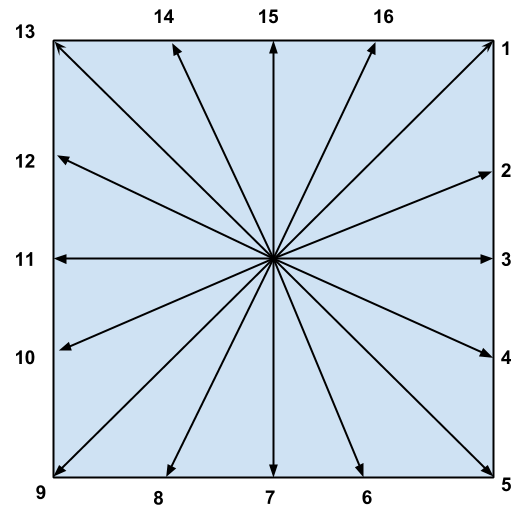
\includegraphics[width=0.9\linewidth]{obrazky/repeatability.png}%
    \caption{Repeatabilita TODO.}
    \label{fig:repeatability}
\end{figure}


